% !TEX root = sum1.tex
\section{Basic Concepts}
In this section, we integrate social distancing measures into the seat planning process. We use the concept of a `pattern' to represent the seat planning, introducing the idea of the `full' and `largest' pattern. Next, we present the deterministic seat planning problem. For seat planning that does not utilize all available seats, we propose to improve the seat planning by incorporating full or largest patterns.

\subsection{Seat Planning with Social Distancing}
We incorporate the social distancing in the seat planning problem. Consider a seat layout comprising $N$ rows, with each row containing $L_j^0$ seats, where $j \in \mathcal{N} \coloneqq \{1,2, \ldots, N\}$. The seating arrangement is used to accommodate various groups, where each group consists of no more than $M$ individuals. There are $M$ distinct group types, denoted by group type $i$, where each group type consists of $i$ people. The set of all group types is denoted by $\mathcal{M} \coloneqq \{1, 2, \ldots, M\}$. The deterministic demand for each group type is represented by a demand vector $\mathbf{d} = (d_1, d_2, \ldots, d_M)^{\intercal}$, where $d_i$ is the demand of group type $i$.


In order to comply with the social distancing requirements, individuals from the same group must sit together, while maintaining a distance from other groups. Let $\delta$ denote the social distancing, which could entail leaving one or more empty seats. Specifically, each group must ensure the empty seat(s) with the adjacent group(s).

To model the social distancing requirements into the seat planning process, we add the parameter, $\delta$, to the original group sizes, resulting in the new size of group type $i$ being denoted as $n_i = i + \delta$, where $i \in \mathcal{M}$. Accordingly, the size of each row is also adjusted to accommodate the adjusted group sizes. Consequently, $L_j = L_j^{0} + \delta$ represents the length of row $j$, where $L_j^{0}$ indicates the number of seats in row $j$. By incorporating the additional seat(s) and designating certain seat(s) for social distancing, we can integrate social distancing measures into the seat planning problem.


We introduce the term pattern to represent the seat planning arrangement for a single row. A specific pattern can be represented by a vector $\bm{h} = (h_1, \ldots, h_M)$, where $h_i$ is the number of group type $i$ in the row for $i = 1,\ldots, M$. A feasible pattern, $\bm{h}$, must satisfy the condition $\sum_{i=1}^{M} h_i n_i \leq L$ and belong to the set of non-negative integer values, denoted as $\bm{h} \in \mathbb{N}^{M}$. Then a seat planning with $N$ rows can be expressed by $\bm{H} = \{\bm{h}_1; \ldots; \bm{h}_N\}$.
  
Let $|\bm{h}|$ indicate the maximum number of people that can be assigned according to pattern $\bm{h}$, i.e., $|\bm{h}| = \sum_{i =1}^{M} i h_i$. The size of $\bm{h}$, $|\bm{h}|$, provides a measure of the maximum number of seats which can be taken due to the implementation of social distancing constraints. By examining $|\bm{h}|$ associated with different patterns, we can assess the effectiveness of various seat planning configurations with respect to accommodating the desired number of individuals while adhering to social distancing requirements.

\begin{example}
Consider the given values: $\delta = 1$, $L^{0} = 10$, and $M = 4$. By adding one seat to each group and the original row, we can realize the conversion, as shown in the following figure.

\begin{figure}[ht]
    \centering
        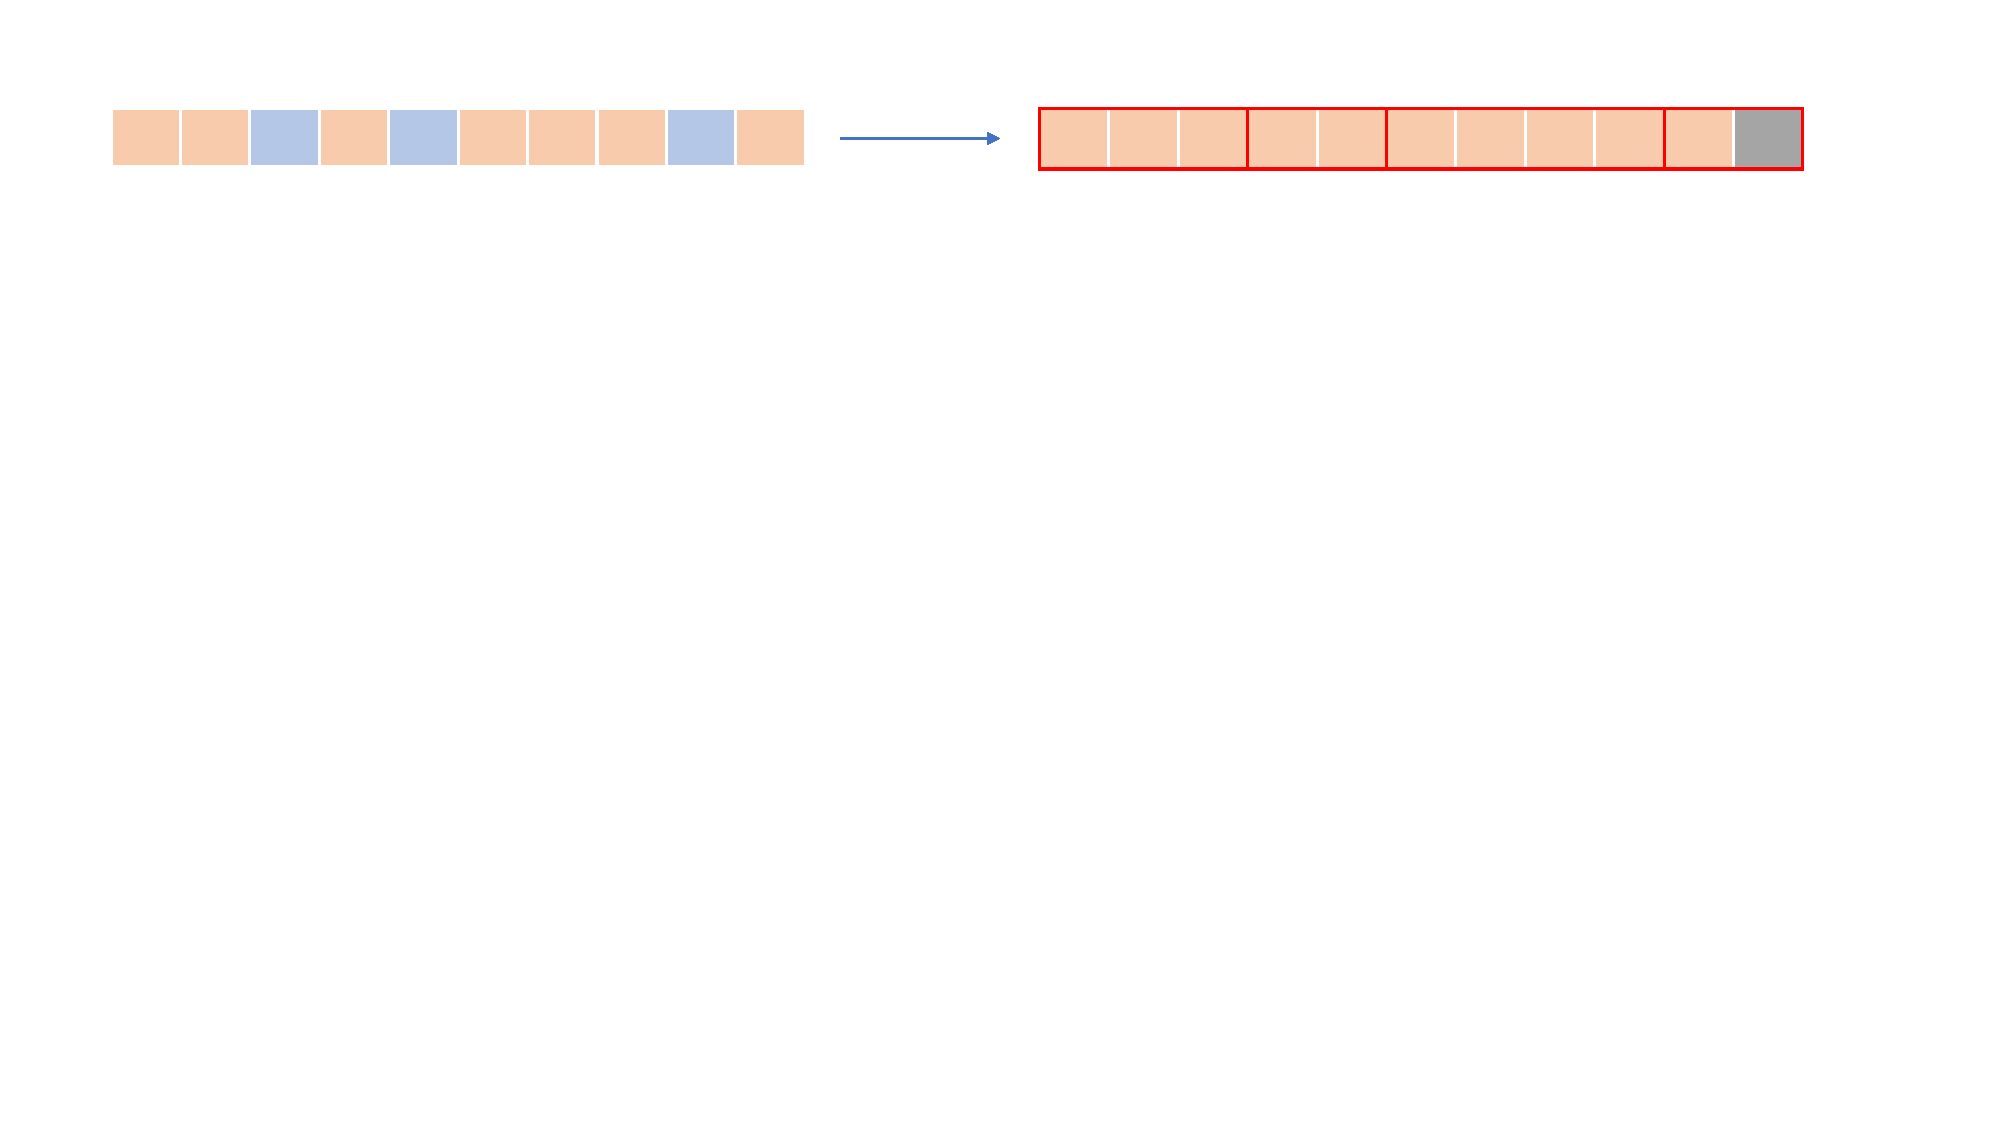
\includegraphics[width=0.8\textwidth]{./Figures/dummy_seat.pdf}
    \caption{Problem Conversion with One Seat as Social Distancing}
\end{figure}

After the conversion, $L = L^{0} + 1 =11$, $n_i = i + 1$ for $i = 1, 2, 3, 4$. For the first group, we use a group of three seats to indicate the original group of two and one seat used as the social distancing. We do the same procedure for the other groups. Then, the row can be represented by $\bm{h} = (2,1,1,0)$. The maximum number of people that can be accommodated is $|\bm{h}| = 7$.
\end{example}


\begin{definition}
Given the length of a row, denoted as $L$, and the maximum size of a group allowed, denoted as $M$, we can define certain characteristics of a pattern $\bm{h} = (h_1, \ldots, h_M)$.
We refer to a pattern $\bm{h}$ as a full pattern if it satisfies the condition $\sum_{i=1}^{M} n_i h_i = L$. Furthermore, we define a feasible pattern $\bm{h}$ as a largest pattern if it has a size $|\bm{h}|$ that is greater than or equal to the size $|\bm{h}^{\prime}|$ of any other feasible pattern $\bm{h}^{\prime}$.
\end{definition}

In other words, a full pattern is one in which the sum of the product of the number of occurrences $h_i$ and the size $n_i$ of each group in the pattern is equal to the length of the row $L$. This ensures that the pattern fully occupies the available row seats. A largest pattern is one that either has the maximum size or is equal in size to other patterns, ensuring that it can accommodate the maximum number of people within the given row length.


\begin{prop}\label{lem_pattern}
Given the parameters of a row, including its length $L$, the social distancing requirement $\delta$, and the number of people in a group allowed $M$, if the size of one feasible pattern $\bm{h}$, is $|\bm{h}| = qM + \max\{r-\delta, 0\}$, where $q = \lfloor \frac{L}{M + \delta} \rfloor$, $r \equiv L \bmod (M + \delta)$, then this pattern is a largest pattern. 
\end{prop}


% The corresponding loss of the largest pattern equals $q \delta - \delta + \min\{r, \delta\}$, represents the amount of empty seats due to the social distancing requirement. 

Proposition \ref{lem_pattern} states that if the size of a pattern is $|\bm{h}| = qM + \max\{r-\delta, 0\}$, then this pattern is the largest pattern. Furthermore, according to the definition of the largest pattern, the size of one possible largest pattern is given by $qM + \max\{r-\delta, 0\}$.

When $r = 0$, the largest pattern $\bm{h}$ is unique and full, indicating that only one pattern can accommodate the maximum number of people. On the other hand, if $r > \delta$, the largest pattern $\bm{h}$ is full, as it utilizes the available space up to the social distancing requirement.

\begin{example}
Consider the given values: $\delta = 1$, $L = 21$, and $M = 4$. In this case, we have $n_i = i + 1$ for $i = 1, 2, 3, 4$. The size of the largest pattern can be calculated as $qM + \max\{r-\delta, 0\} = 4 \times 4 + 0 = 16$. The largest patterns are the following: $(1, 0, 1, 3)$, $(0, 1, 2, 2)$, $(0, 0, 0, 4)$, $(0, 0, 4, 1)$, and $(0, 2, 0, 3)$.

The following figure shows that the largest pattern may not be full and the full pattern may not be largest.
\begin{figure}[ht]
    \centering
        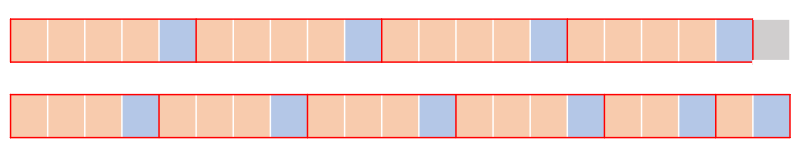
\includegraphics[width=0.8\textwidth]{./Figures/full_largest.png}
    \caption{Full and Largest Pattern}
\end{figure}

The first row can be represented by $(0, 0, 0, 4)$. It is a largest pattern as it can accommodate the maximum number of individuals. However, it does not satisfy the requirement of fully utilizing all available seats since $4 \times 5 \neq 21$.
The second row can be represented by $(1, 1, 4, 0)$, which is a full pattern as it utilizes all available seats. However, its size is 15, indicating that it is not a largest pattern.
\end{example}

\subsection{Seat Planning Problem}
Let $x_{ij}$ represent the number of group type $i$ planned in row $j$. The deterministic seat planning problem is formulated below, with the objective of maximizing the number of people accommodated.

\begin{equation}\label{deter_upper}
    \begin{aligned}
    \max \quad & \sum_{i=1}^{M}  \sum_{j= 1}^{N} (n_i- \delta) x_{ij} \\
    \text {s.t.} \quad & \sum_{j= 1}^{N} x_{ij} \leq d_{i}, \quad i \in \mathcal{M}, \\
    & \sum_{i=1}^{M} n_{i} x_{ij} \leq L_j, j \in \mathcal{N}, \\
    & x_{ij} \in \mathbb{N}, \quad i \in \mathcal{M}, j \in \mathcal{N}.
    \end{aligned}
\end{equation}
  
This seat planning problem can be regarded as a special case of the multiple knapsack problem. In this context, we define $\bm{X}$ as the aggregate solution, where $\bm{X} = (\sum_{j=1}^{N} x_{1j}, \ldots, \sum_{j=1}^{N} x_{Mj})^T$. Each element of $\bm{X}$, $\bm{X}_{i} = \sum_{j=1}^{N} x_{ij}$, represents the available supply for group type $i$.
  
In other words, $\bm{X}$ captures the number of each group type that can be allocated to the seat layout by summing up the supplies across all rows. By considering the monotone ratio between the original group sizes and the adjusted group sizes, we can determine the upper bound of supply corresponding to the optimal solution of the LP relaxation of Problem \eqref{deter_upper}, as demonstrated in Proposition \ref{sol_relax_deter}.

% Although the problem size is small and the optimal solution can be easily obtained by using a solver, it is still important to analyze the problem further to gain additional insights and understanding.

% In many cases, the optimal solution for the seat planning problem tends to involve rows with either full patterns or the largest patterns. Distinguishing these patterns from other configurations can provide valuable insights into effective seat planning strategies that prioritize accommodating as many people as possible while adhering to social distancing guidelines.

% When there is high demand for seats, it is advantageous to prioritize the largest patterns. These patterns allow for the accommodation of the largest number of individuals due to social distancing requirements. On the other hand, in scenarios with moderate demand, adopting the full pattern becomes more feasible. The full pattern maximizes seating capacity by utilizing all available seats, except those empty seats needed for social distancing measures. By considering both the largest and full patterns, we can optimize seat planning configurations to efficiently accommodate a significant number of individuals while maintaining adherence to social distancing guidelines. 


% Although the optimal solution to the seat planning problem is complex, the LP relaxation of problem \eqref{deter_upper} has a nice property.

\begin{prop}\label{sol_relax_deter}
For the LP relaxation of problem \eqref{deter_upper}, there exists an index $\tilde{i}$ such that the optimal solutions satisfy the following conditions: $x_{ij}^{*} = 0$ for all $j$, $i = 1,\ldots, \tilde{i}-1$; $\sum_{j} x_{ij}^{*} = d_{i}$ for $i = \tilde{i}+1,\ldots, M$; $\sum_{j} x_{ij}^{*} = \frac{L - \sum_{i = \tilde{i}+1}^{M} {d_i n_i}}{n_{\tilde{i}}}$ for $i = \tilde{i}$.
\end{prop}


For $i = 1,\ldots, \tilde{i}-1$, $x_{ij}^{*} = 0$ for all rows, indicating that no group type $i$ are assigned to any rows before index $\tilde{i}$. For $i = \tilde{i}+1,\ldots, M$, the optimal solution assigns $\sum_{j} x_{ij}^{*} = d_{i}$ group type $i$ to meet the demand for group type $i$. For $i = \tilde{i}$, the optimal solution assigns $\sum_{j} x_{ij}^{*} = \frac{L - \sum_{i = \tilde{i}+1}^{M} {d_i n_i}}{n_{\tilde{i}}}$ group type $\tilde{i}$ to the rows. This quantity is determined by the available supply, which is calculated as the remaining seats after accommodating the demands for group types $\tilde{i}+1$ to $M$, divided by the size of group type $\tilde{i}$, denoted as $n_{\tilde{i}}$.

Hence, the corresponding supply associated with the optimal solutions can be summarized as follows: $X_{\tilde{i}} = \frac{L - \sum_{i = \tilde{i}+1}^{M} {d_i n_i}}{n_{\tilde{i}}}$, $X_{i} = d_{i}$ for $i = \tilde{i} +1,\ldots, M$, and $X_{i} = 0$ for $i = 1, \ldots, \tilde{i}-1$.

\subsection{Generate The Seat Planning Composed of Full or Largest Patterns}
The seat planning obtained from problem \eqref{deter_upper} may not utilize all available seats, as it depends on the given demand. To improve a given seat planning and utilize all seats, we aim to generate a new seat planning that can assign the maximum number of seats to the possible groups while ensuring that the original group type requirements are met.

We seek to find a seat planning $\bm{H}^{\prime}$ for any feasible seat planning $\bm{H}$.Specifically, we reallocate the seats to obtain a seat planning, $\bm{H}^{\prime}$, which can satisfy the realized demand $\sum_{j=1}^{N} H_{ji}$ for each group type $i$. Mathematically, we can solve the following programming to obtain the improved seat planning:

\begin{equation}\label{improve_seat}
  \begin{aligned}
  \max \quad & \sum_{i=1}^{M} \sum_{j=1}^{N} (n_i-\delta)  x_{ij} \\
  s.t. \quad & \sum_{j=1}^{N} \sum_{k=i}^{M} x_{kj} \geq  \sum_{k=i}^{M} \sum_{j=1}^{N} H_{ji}, i \in \mathcal{M} \\
  & \sum_{i=1}^{M} n_{i} x_{ij} \leq L_{j}, j \in \mathcal{N} \\
  & x_{ij} \in \mathbb{N}, i \in \mathcal{M}, j \in \mathcal{N}
  \end{aligned}
\end{equation}

Since smaller groups can be satisfied by larger groups, for each group type $i$, the total quantity from group $i$ to group $M$ should be no less than the total satisfied demand from group type $i$ to group type $M$, as shown in the first set of constraints in problem \eqref{improve_seat}. The optimal solution obtained from problem \eqref{improve_seat} represents the desired seat planning $\bm{H}^{\prime}$ and each pattern in $\bm{H}^{\prime}$ is either largest or full.

\begin{prop}\label{prop_construction}
  Problem \eqref{improve_seat} can always generate a seat planning $\bm{H}^{\prime}$ composed of full or largest patterns, given a feasible seat planning $\bm{H}$.
\end{prop}

This approach guarantees efficient seat allocation, maximizing the utilization of available seats while still accommodating the original groups' requirements. Furthermore, the improved seat planning can be used for the seat assignment when the demand arrives sequentially.

% When there is high demand for seats, it is advantageous to prioritize the largest patterns. These patterns allow for the accommodation of the largest number of individuals due to social distancing requirements. On the other hand, in scenarios with moderate demand, adopting the full pattern becomes more feasible. The full pattern maximizes seating capacity by utilizing all available seats, except those empty seats needed for social distancing measures. By considering both the largest and full patterns, we can optimize seat planning configurations to efficiently accommodate a significant number of individuals while maintaining adherence to social distancing guidelines. 



% Instead of solving the above programming directly, we can follow this approach to find the desired pattern $\bm{h}^{\prime}$. Let $\beta_{j}= L_{j} - \sum_{i} n_{i} x_{ij}$ for each row $j$, where $\beta_{j}$ represents the remaining unoccupied seats. Our goal is to allocate these remaining seats, $\beta_{j}$, to the previously planned groups to make them as large as possible. If there are still unoccupied seats available after this, we aim to allocate them to new largest groups as many as possible.

% Now, we demonstrate the specific allocation scheme. Find the smallest group type in the pattern denoted as $k$. If $k = M$, it means that this row corresponds to a largest pattern. If $k \neq M$, we reduce the number of group type $k$ by one and increase the number of group type $\min \{(k+\beta_{j}), M\}$ by one, the number of unoccupied seats will be reduced correspondingly.

% We continue this procedure until either all the planned groups become the largest or $\beta_{j} = 0$. If $\beta_{j} = 0$, it indicates that the pattern is full. In this case, we have assigned all the unoccupied seats to the existing groups. Therefore, this full pattern has the largest size while satisfying the groups requirement. However, if all the planned groups become the largest and $\beta_{j} \neq 0$, we can repeatly follow the steps outlined below to obtain the largest pattern:


% \begin{itemize}
%   \item If $\beta_{j} \geq n_{M}$, we can assign $n_M$ seats to a new group type $M$.

%   \item If $n_{1} \leq \beta_{j} < n_{M}$, we can assign $\beta_{j}$ seats to a new group type $\beta_{j}-n_{1}+1$.
%   \item If $0 < \beta_{j} < n_{1}$, it means that the current pattern is already the largest possible pattern because all the planned groups in the pattern are the largest.
% \end{itemize}


% \begin{algorithm}
%   \caption{Construct The Largest or Full Pattern for Row $j$}\label{construction}
%   % \KwIn{Pattern $\bm{h}$}
%   % \KwOut{Pattern}
%   \While{$\beta_j > 0$}
%     {$k \gets \min_{i}\{h_{i} \neq 0\}$\Comment*[r]{Find the smallest group type in the pattern}
%     \eIf{$k \neq M$}
%     {$h_{k} \gets h_{k} - 1$\; $h_{\min\{k+\beta_j, M\}} \gets h_{\min\{k+\beta_j, M\}} + 1$\;
%     $\beta_j \gets \beta_j - \max\{1, M - k\}$\Comment*[r]{Change the current group type to a group type as large as possible}}
%     {\eIf{$\beta_j \geq n_{M}$}
%     {$q \gets \lfloor\frac{\beta_j}{n_M}\rfloor$\;
%      $\beta_j \gets \beta_j - q \cdot n_M$\; $h_{M} \gets h_{M} + q$\Comment*[r]{Assign seats to as many the largest group type as possible}}
%     {\eIf{$n_{1} \leq \beta_j < n_{M}$}
%     {$h_{\beta_j-n_1+1} \gets h_{\beta_j-n_1+1} + 1$\; $\beta_j \gets 0$\;}
%     {$\bm{h}$ is the largest\; $\beta_j \gets 0$\;}}
%     }}
% \end{algorithm}


% Since patterns are independent of each other, we can employ Algorithm row by row within a given seat planning. This enables us to optimize the seat planning by maximizing the utilization of available seats.

% By following these steps and always prioritizing the largest group type for seat planning, we can achieve the largest or full pattern. This approach guarantees efficient seat allocation, maximizing the utilization of available seats while still accommodating the original groups' requirements. To construct the largest or full pattern for each row, we can employ the following algorithm.

